\documentclass{article}
\usepackage{crysymb}
\usepackage[draft]{crygame}
\usepackage{crypto-ii}
\usepackage{graphics}
\usepackage{graphicx}


\begin{document}

\noindent	
MTAT.07.003 Cryptology II\\
Spring 2016 / Exercise session IV 


\subsection*{PRP/PRF switching lemma}

\centerline{ 
  \includegraphics[angle=-90, scale=0.45, trim=0.0cm 2.5cm 13.0cm
  0.5cm,clip=true]{illustrations/switching-lemma.eps}}


\begin{enumerate}

\item Let $\AD$ be the adversary that tries to distinguish a random
  permutation $f:\set{1,2,3}\to\set{1,2,3}$ from a random function
  $f:\set{1,2,3}\to\set{1,2,3}$ according to the adaptive
  deterministic querying strategy depicted above. More formally, nodes
  represents adversaries queries. The adversary $\AD$ starts form the
  root node and moves to next nodes according to the answers depicted
  as arc labels.  The dashed line corresponds to the decision border,
  where $\AD$ stops querying and outputs his or her guess.
  \begin{enumerate}
  \item Compute the following probabilities 
    \begin{align*}
      &\pr{f\gets\FFFALL:\text{$\AD$ reaches vertex $u$}}\enspace,\\
      &\pr{f\gets\FFFALL:\text{$\AD$ reaches vertex $u\wedge \neg\mathsf{Collision}$}}\enspace,\\
      &\pr{f\gets\FFFALL:\text{$\neg\mathsf{Collision}$}}\enspace,\\
      &\pr{f\gets\FFFALL:\text{$\AD$ reaches vertex $u| \neg\mathsf{Collision}$}}\enspace,\\
      &\pr{f\gets\FFFPERM:\text{$\AD$ reaches vertex $u$}}
    \end{align*}
    for all nodes $u$ in the decision border.
  \item Compute these probabilities for an arbitrary message space
    $\MSPACE$ under the assumption that $\AD$ makes exactly $q$
    queries and conclude
    \begin{align*}
      \pr{\AD=0|\FFFALL\wedge\neg\mathsf{Collision}}=\pr{\AD=0|\FFFPERM}\enspace.
    \end{align*}
  \end{enumerate}

\item For the proof of the PRP/PRF switching lemma, consider the
  following games.  In the game $\GAME_0$, the challenger first draws
  $f\gets\FFFALL$ and then answers up to $q$ distinct queries. In the
  game $\GAME_1$, the challenger draws $f\gets\FFFPERM$ and then
  answers up to $q$ distinct queries. In both games, the output is
  determined by the adversary $\AD$ who submits its final verdict.
  \begin{enumerate}
  \item Formalise both games as short programs, where $\GAME$ can make
    oracle calls to $\AD$. For example, something like
    \begin{align*}
      \begin{game}{\GAME_0^\AD}
        &f\getsu\FFFALL\\
        & y_0\gets \bot\\
        &\begin{fblock}{\text{For $i\in\set{1,\ldots,q}$ do}}
        & x_i\gets\AD(y_{i-1})\\
        &\text{If $x_i=\bot$ then break the cycle}\\
        & y_i\gets f(x_i)
        \end{fblock}\\
        &\RETURN \AD
      \end{game}
    \end{align*}
  \item Rewrite both games so that there are no references to the
    function $f$ but the behaviour does not change. Denote these games
    by $\GAME_2,\GAME_3$.
  \item Analyse what is the probability that execution in the games
    $\GAME_2$ and $\GAME_3$ starts to diverge. Conclude
    $\SD_\star(\GAME_2,\GAME_3)=\pr{\mathsf{Collision}}$
  \end{enumerate}
  \textbf{Hint:} Note that following code fragment samples uniformly
  permutations
  \begin{align*}
    \begin{fblock}{\text{Sample $f(x_i)$}}
      &y_i\getsu\MSPACE\\
      &\begin{fblock}{\text{If $y_i\in\set{y_1,\ldots,y_{i-1}}$ then}}
        y_i\getsu\MSPACE\setminus\set{y_1,\ldots,y_i}
      \end{fblock}
    \end{fblock}
  \end{align*}
  What is the probability we ever reach the if branch?

   

\item Let $y_1,\ldots,y_q$ be chosen uniformly and independently from
  the set $\MSPACE$. Let $\mathsf{Distinct}(k)$ denote the event that
  $y_1,\ldots,y_k$ are distinct. Estimate the value of
  $\pr{\mathsf{Distinct}(k)|\mathsf{Distinct}(k-1)}$ and this result
  to prove
  \begin{align*}
    \pr{\mathsf{Distinct}(k)}\leq e^{-q(q-1)/(2\abs{\MSPACE})}
  \end{align*}
   How one can use this result to prove the birthday bound
   \begin{align*}
     \pr{\mathsf{Collision}|q \text{ queries}}\geq 0.316\cdot
     \frac{q(q-1)}{\abs{\MSPACE}}\enspace.
   \end{align*}
  \textbf{Hint:} Note that $1-x\leq e^{-x}$. \\
  \textbf{Hint:} Note that $1-e^{-x}\geq (1-e^{-1})x$ if $x\in[0,1]$.

\item A block cipher is commonly modelled as a
  $(t,q,\varepsilon)$-pseudorandom permutation family $\FFF$. As
  such, it is perfect for encrypting a single block.
  \begin{enumerate}
  \item The electronic codebook mode $\textsc{Ecb}$ uses a same
    permutation $f\gets\FFF$ for all message blocks
    $\textsc{Ecb}_f(m_1\|\ldots\|m_n)= f(m_1)\|\ldots\| f(m_n)$ is
    known to be insecure pseudorandom permutation.  Find an algorithm
    that can distinguish $\textsc{Ecb}_f:\MSPACE^n\to\MSPACE^n$ from a
    random permutation over $\MSPACE^n$. Is this weakness relevant in
    practise or not?
  \item Let $\MSPACE_\circ^n=\set{(m_1,\ldots,m_n)\in\MSPACE^n:
      m_i\neq m_j}$ denote the set of messages with distinct
    blocks. Show that
    $\textsc{Ecb}_f:\MSPACE_\circ^n\to\MSPACE_\circ^n$ is
    $(t,\frac{q}{n},\varepsilon)$-pseudorandom permutation family if
    $\FFF$ is $(t,q,\varepsilon)$-pseudorandom permutation family.
  \item If addition is defined over $\MSPACE$, random shifts
    $c_1,\ldots,c_n\getsu\MSPACE$ can be used to avoid equalities in
    the message $\overline{\vec{m}}=(m_1+c_1,\ldots,m_n+c_n)$. Compute
    the probability $\pr{c_1,\ldots,c_n\getsu\MSPACE:
      \overline{\vec{m}}\notin\MSPACE_\circ^n}$.
  \item The cipher-block chaining mode $\textsc{Cbc}$ uses the
    permutation $f\gets\FFF$ to link plaintext and ciphertexts:
    $\textsc{Cbc}_f(m_1\|\ldots\|m_n)= c_1\|\ldots\|c_n$ where
    $c_i=f(m_i\oplus c_{i-1})$ and $c_0$ is know as initialisation
    vector (nonce).  The $\textsc{Cbc}$ mode can be viewed as more
    efficient way to modify the message by setting shifts $c_{i}\gets
    f(\overline{m}_{i-1})$. Again, compute the probability
    $\pr{c_0\getsu\MSPACE,\cdots, c_n\gets
      f(m_{n-1}+c_{n-1}):\overline{\vec{m}}\notin\MSPACE_\circ^n}$.
    Conclude that $\textsc{CBC}_f$ is a secure pseudorandom
    permutation over $\MSPACE^n$.
  \end{enumerate}
\item The IND-CPA security notion is also applicable for symmetric
  cryptosystems. Namely, a symmetric cryptosystem $(\GEN,\ENC,\DEC)$
  is $(t,\varepsilon)$-IND-CPA secure, if for any $t$-time adversary
  $\AD$:
  \begin{align*}
    \advINDCPAXX{}{\AD}=\abs{\pr{\smash{\GAME_0^\AD=1}}-\pr{\smash{\BGAME_1^\AD=1}}}\leq
    \varepsilon
  \end{align*}
 where
  \begin{align*}
    \begin{game}{\BGAME_0^\AD}
      &\SK\gets\GEN\\
      &(m_0,m_1)\gets\AD^{\ORA_1(\cdot)}\\
      &\RETURN \AD^{\ORA_1(\cdot)}(\ENC_\SK(m_0))
    \end{game}
    \qquad\qquad
     \begin{game}{\BGAME_1^\AD}
      &\SK\gets\GEN\\
      &(m_0,m_1)\gets\AD^{\ORA_1(\cdot)}\\
      &\RETURN \AD^{\ORA_1(\cdot)}(\ENC_\SK(m_1))
    \end{game}
  \end{align*}
  and the oracle $\ORA_1$ serves encryption calls.
  
  Let $f:\MSPACE\times\KSPACE\to\MSPACE$ be a
  $(t,\varepsilon)$-pseudorandom permutation. Then a $\textsc{Ctr-\$}$
  symmetric encryption scheme is defined as follows:
  \begin{itemize}
  \item A secret key is a randomly chosen $k\getsu\KSPACE$.
  \item To encrypt a message $m_1,\ldots,m_n$, choose a random nonce
    $s_0\getsu\MSPACE$ and output $s_0,m_1+f(s_0+1,k),\ldots,
    m_n+f(s_0+n,k)$.
  \item To decrypt $s_0,c_1,\ldots,c_n$, output $c_1-f(s_0+1,k),\ldots,c_n-f(s_0+n,k)$.
  \end{itemize}
  Prove that $\textsc{Ctr-\$}$ is IND-CPA secure cryptosystem.


\item Estimate computational distance between following games under
  the assumption that $(\GEN,\ENC,\DEC)$ is $(t,\varepsilon)$-IND-CPA
  secure cryptosystem.
  \begin{enumerate}
  \item Left-or-right games
    \begin{align*}
      \begin{game}{\GAME_0^\AD}
      &\SK\gets\GEN\\
      &\begin{fblock}{\text{For $i=1,\ldots,q$ do}}
      &(m_0^i,m_1^i)\gets\AD\\
      &\text{Give $\ENC_\SK(m_0^i)$ to $\AD$}
      \end{fblock}\\
      &\RETURN \text{the output of }\AD
      \end{game}
      \qquad\qquad
      \begin{game}{\GAME_1^\AD}
      &\SK\gets\GEN\\
      &\begin{fblock}{\text{For $i=1,\ldots,q$ do}}
      &(m_0^i,m_1^i)\gets\AD\\
      &\text{Give $\ENC_\SK(m_1^i)$ to $\AD$}
      \end{fblock}\\
      &\RETURN \text{the output of }\AD
      \end{game}
     \end{align*}
   \item Real-or-random games
    \begin{align*}
      \begin{game}{\GAME_0^\AD}
      &\SK\gets\GEN\\
      &\begin{fblock}{\text{For $i=1,\ldots,q$ do}}
      &m^i\gets\AD\\
      &\text{Give $\ENC_\SK(m^i)$ to $\AD$}
      \end{fblock}\\
      &\RETURN \text{the output of }\AD
      \end{game}
      \qquad\qquad
      \begin{game}{\GAME_1^\AD}
      &\SK\gets\GEN\\
      &\begin{fblock}{\text{For $i=1,\ldots,q$ do}}
      &m_0^i\gets\AD,m_1^i\getsu\MSPACE\\
      &\text{Give $\ENC_\SK(m_1^i)$ to $\AD$}
      \end{fblock}\\
      &\RETURN \text{the output of }\AD
      \end{game}
     \end{align*}
  \end{enumerate}




\end{enumerate}


\end{document}